\chapter{Investigación de plataformas Blockchain} % Main chapter title

\label{Chapter2} % Change X to a consecutive number; for referencing this chapter elsewhere, use \ref{ChapterX}

\lhead{Capítulo 2. \emph{Investigación de plataformas Blockchain}} % Change X to a consecutive number; this is for the header on each page - perhaps a shortened title
\setstretch{1.1} % Line spacing of 1.1
El presente capítulo introduce conceptos generales sobre Blockchain. Luego, se plantean los primeros requerimientos tentativos en base al conocimiento adquirido. Por último, se estudian implementaciones actuales de Blockchain y se analiza su utilidad para el proyecto integrador.

%----------------------------------------------------------------------------------------
%	SECTION 1
%----------------------------------------------------------------------------------------

\section{Bitcoin}

La mejor forma de comprender la tecnología Blockchain y el potencial que tiene es estudiando su primera implementación: Bitcoin. En el \textit{paper}, “Research Perspectives and Challenges for Bitcoin and Cryptocurrencies”\cite{7163021}, los autores extraen 3 componentes principales de la tecnología novedosa:

\subsection{Transacciones y scripts}
En Bitcoin, una cuenta de usuario es representada por un conjunto de clave pública y privada. El \textit{hash} de la clave pública funciona como número de cuenta a la cual se puede enviar dinero.
Las transferencias de Bitcoin, de forma simplificada, consisten en un conjunto de entradas y un conjunto de salidas de monedas asociadas a los números de cuenta mencionados. El movimiento de dinero se puede entender como flujos, que se dividen o unen con cada transferencia realizada. Las salidas como entradas están vinculados a \textit{scripts} que se tienen que ejecutar de forma correcta para que la operación sea declarada válida. El contenido de dichos \textit{scripts} puede ser complejo, pero en transacciones comunes suele contener solamente comandos de validación de firma.
\subsection{La red \textit{peer to peer}}
Cualquier PC con acceso a Internet puede unirse a la red Bitcoin. El participante nuevo establece conexiones con una cantidad aleatoria de otros participantes. Luego, información como bloques nuevos o transacciones pendientes son distribuidos vía \textit{broadcast} e inundación. Además, el protocolo Bitcoin contiene varios mecanismos de seguridad: Cada nodo reenvía paquetes una sola vez para evitar bucles infinitos debido a la inundación. Transferencias de montos muy pequeños pueden ser usados para \textit{penny-flooding attacks}, por lo cual nodos limitan la retransmisión de dichas transferencias por segundo.
\subsection{Consenso y minado}
Cuando un participante de la red realiza una transacción y la transmite a la red vía \textit{broadcast}, esta tiene que ser validada y almacenada. Para lograr eso sin necesidad de un ente centralizado, Bitcoin usa varios mecanismos en conjunto.
\begin{itemize}
\item El Blockchain: Nodos especiales llamados mineros agrupan transacciones realizadas en bloques de un cierto tamaño, por ejemplo de 1 Megabyte en Bitcoin. Luego agregan el \textit{hash} del bloque anterior a su bloque, enlazando así la información y formando una cadena de bloques con transacciones. 

\item Un mecanismo de consenso: El Blockchain es el registro de todas las transferencias realizadas de toda la red ordenadas en el tiempo. Cada nodo de la red tiene una copia idéntica almacenada. Por ende, todos los participantes tienen que estar de acuerdo sobre cuál es la versión válida y actual. No puede haber divisiones - si mineros publican 2 bloques al mismo tiempo y por latencias en la red hay nodos que agregan el bloque A y otros que agregan el bloque B, se produce lo que se llama \textit{fork}. El protocolo está diseñado para que, después de un tiempo, todos los nodos opten por la misma rama.

\item \textit{Proof of Work}: Es el elemento esencial gracias al cual el Blockchain se vuelve inmutable y se llega al consenso descrito en el punto 2. Antes de poder publicar un bloque para que forme parte del Blockchain, cada minero realiza un cálculo computacional complejo, cuyo resultado es agregado al bloque y resulta fácil de verificar por otros. La dificultad del cálculo está definida en el código para que un bloque sea publicado cada 10 minutos en promedio. En el caso de una división, la red decide por la rama con el mayor \textit{Proof of Work} acumulado. El mecanismo también resuelve otros problemas: como la publicación de un bloque es costosa en términos de capacidad de procesamiento, se evita que un nodo malintencionado produzca un \textit{spam} de bloques. La secuencia forzada y el abandono de ramas debido a \textit{forks} logra mantener transacciones coherentes en el Blockchain. %y evita que un participante pague dos veces con el mismo dinero \textit{(double spending attack)}.%
Por último, asegura la inmutabilidad del Blockchain: si un minero quiere insertar una transacción fraudulenta en el bloque 4 de una cadena de 6 bloques, es necesario volver a computar el \textit{Proof of Work} de los bloques 4, 5 y 6 antes de que otro minero adjunte el bloque nro. 7 a la cadena original.

Una de las desventajas principales de \textit{Proof of Work} consiste en la competencia entre los mineros: En un instante dado, todos los mineros están trabajando para obtener resultado del cálculo complejo, pero solo el primero en obtenerlo puede adjuntar el bloque nuevo al Blockchain. Los otros tienen que abortar su cálculo, ensamblar un bloque nuevo y volver a empezar. Eso ha llevado a críticas por el consumo de energía eléctrica de la red Bitcoin: En Agosto del 2018, el consumo del año 2018 fue estimado en 73,12 TWh - la cantidad de energía que necesita la población completa de Austria durante un año.\cite{bitcoin_energy}.

\end{itemize}

Una vez que Bitcoin ganó popularidad, se dieron dos tendencias: por un lado, muchos programadores lanzaron otras criptomonedas modificando el código fuente de Bitcoin. Las criptomonedas alternativas recibieron el nombre \textit{altcoin} y en Agosto del 2018 se listan 1855 \textit{altcoins} en total\cite{altcoins}. Por otro lado, desarrolladores vieron posibilidades más allá de las criptomonedas e implementaron productos con tecnología Blockchain cuyos enfoques no se limitan a monedas digitales. Más adelante se van a analizar varios de esos productos.

\section{Primeras especificaciones para el prototipo}
\label{sec:primeras_especificaciones_prototipo}

Luego de analizar el funcionamiento de Bitcoin, Blockchain no aparenta ser una solución conveniente para los problemas planteados en el capítulo anterior. Una arquitectura que se basa en la ausencia de confianza y una base de datos que requiere de la competencia de mineros para volverse inmutable, no parece adecuarse a un sistema estructurado con autoridades centrales como la universidad. 

Si bien implementar un prototipo de un sistema de distribución de información académica en Bitcoin no aporta mucho valor - dado desventajas evidentes como la posible participación de cualquier persona en el mundo - implementar dicho prototipo en un Blockchain tiene sentido, siempre y cuando las necesidades de la universidad concuerdan con la arquitectura del sistema.

Por eso, a continuación, se detallan las limitaciones del Blockchain de Bitcoin junto con las modificaciones correspondientes que deben tenerse en cuenta para que la elección de un Blockchain como solución resulta ser conveniente:

\begin{itemize}


\item \textbf{Control de Acceso} \newline

Para formar parte de la red Bitcoin, sólo es necesario instalar un software en una computadora y crear una cuenta. No existen restricciones de acceso, la participación es anónima y cualquier nodo puede inspeccionar el historial completo de las transferencias. 
Para el caso del prototipo planteado, dichas características son indeseadas: el acceso de entidades ajenas debe estar restringido y la información debe ser visible únicamente por las partes autorizadas. Eso implica que es necesario conocer identidades y controlar sus accesos al Blockchain. 
Existen 2 modelos para el caso descrito: Blockchains privados y Blockchains de consorcio.

\begin{quote}Un Blockchain totalmente privado es un Blockchain donde los permisos de escritura se mantienen centralizados en una organización. Los permisos de lectura pueden ser públicos o restringidos en una extensión arbitraria.\cite{bc_privado}
\end{quote}

\begin{quote}
    Un Blockchain de consorcio es un Blockchain donde el proceso de consenso es controlado por un conjunto de nodos preseleccionados.\cite{bc_privado}
\end{quote}

Como la información debe ser escrita y accedida desde diferentes facultades o eventualmente universidades, un Blockchain de consorcio es la opción más conveniente para el prototipo.

\item \textbf{Privacidad de la información}

En el caso de Blockchains de consorcio o Blockchains privados, el acceso está limitado a las partes autorizadas. Sin embargo, todas las partes autorizadas tienen acceso equitativo a toda la información. Si se desea compartir ciertos datos y mantener otros en privado, se necesita un sistema que otorga derechos de lectura y escritura individuales para cada participante.

\item \textbf{Simplificación del consenso}

El proceso de minado en conjunto con el mecanismo criptográfico \textit{Proof of Work} establece confianza entre partes desconocidas y logra la inmutabilidad de las transferencias en Bitcoin. Dicho trabajo es realizado por nodos mineros que compiten entre ellos para validar transacciones, calcular \textit{Proof of Work} y ganar recompensas monetarias.

Para un Blockchain de consorcio que almacena información académica, dicho mecanismo presenta una solución ineficiente: ya existe un cierto grado de confianza entre los participantes, por lo cual una competencia entre nodos mineros se vuelve innecesaria. El alto consumo energético que eso implica puede resultar un impedimento para la adaptación de la tecnología.

Una alternativa adopción más conservadora con el uso de recursos computacionales es el mecanismo \textit{Proof of Stake}:
\begin{quote}
Protocolos de criptomonedas que intentan evitar el desperdicio de recursos físicos escasos comúnmente confían en \textit{proof of stake}, es decir, en mecanismos que dan poder de decisión con respecto a la continuación del \textit{ledger} a entidades que poseen monedas dentro del sistema.\cite{DBLP:journals/corr/BentovGM14}
\end{quote}
Es decir, el creador de un bloque nuevo es elegido de forma aleatoria. Para poder distinguir ambos mecanismos, se dice que bloques nuevos son forjados y no minados. Dependiendo de la implementación, diferentes parámetros como antigüedad o riqueza pueden favorecer en el momento de la elección del nodo forjador. 

\item \textbf{Reducción de costos transaccionales}

Mineros en Bitcoin son recompensados por asegurar al Blockchain con sus recursos: Por cada bloque publicado, un minero recibe tarifas de las transacciones que validó y una recompensa adicional establecida por el protocolo llamada \textit{block reward}.
\begin{quote}
El principal gasto que debe pagar un Blockchain es la seguridad. El Blockchain debe pagar a los mineros o validadores para que participen económicamente en su protocolo de consenso, ya sea prueba de trabajo o prueba de participación, y esto inevitablemente tiene algún costo. Hay dos formas de pagar este costo: inflación y tarifas de transacción.\cite{bc_tarifas}
\end{quote}
Ambos costos tienen desventajas para empresas:  
Transacciones tarifadas significan un gasto adicional para una empresa que se eleva con la cantidad de transacciones realizadas. En su peor caso pueden inhibir el uso de la tecnología.

El empleo de un \textit{block reward} significa que se crean criptomonedas con cada bloque nuevo que se agrega al Blockchain. De esta forma, la cantidad total de monedas sube constantemente. Una empresa tiene que tener en cuenta el impacto que va a tener dicha inflación en el futuro.

Debido a las complicaciones mencionadas, se busca una solución que logre asegurar el Blockchain con métodos alternativos. Para el caso del prototipo a implementar, la mejor opción es usar un Blockchain sin criptomoneda.

\item \textbf{Automatización}
			 	 	
Los \textit{Smart contracts} fueron implementados por primera vez en Ethereum, la implementación de Blockchain que siguió a Bitcoin: se trata de código que se ejecuta automáticamente cuando se cumplen ciertas condiciones. Son usados por ejemplo por la aplicación Crypto Sportz que automatiza así el pago de apuestas deportivas:
\begin{quote}
Cuando se ingresen los resultados del juego en el contrato, [este] reconocerá los boletos con la predicción correcta como boletos ganadores y dividirá su saldo ETH por el número de boletos ganadores.\cite{crypto_sportz}
\end{quote}
Aplicaciones que funcionan con \textit{smart contracts}, forman una capa de abstracción ``por encima'' del Blockchain, similar a la capa de aplicación en TCP/IP. Los \textit{smart contracts} reciben parámetros y escriben transacciones en el Blockchain. Así se pueden automatizar operaciones específicas.
Si bien la lógica de negocios suele estar embebida en la aplicación, \textit{smart contracts} pueden ayudar a autorizar accesos de lectura y escritura o controlar la validez de información a escribir. Por sus posibilidades de automatización, es deseado que el prototipo a implementar permita escribir \textit{smart contracts}.
\end{itemize}

Dado que en el presente proyecto integrador se quiere emplear una aplicación usando Blockchain y no construir un Blockchain nuevo, es conveniente partir de un código \textit{open source} que se pueda modificar o utilizar un SDK que permite configurar el Blockchain para que cumpla con los requisitos mencionados. Para encontrar una opción conveniente, se estudiaron algunas implementaciones existentes que ofrecen características más allá de una criptomoneda: El criterio de selección de las plataformas a estudiar fue que la idea del desarrollo no se enfoque principalmente en la criptomoneda, sino en funcionalidades adicionales que podrían ser de utilidad para el prototipo a implementar. A continuación se describe cada una de las opciones junto con sus ventajas y desventajas para la implementación del prototipo.

\section{Ethereum}

Ethereum es una plataforma creada por el programador Vitalik Buterin, miembro activo en la comunidad Bitcoin desde 2011.\cite{bitcoinmagazine}
Buterin vio la posibilidad de utilizar la tecnología Blockchain para propósitos más allá de las criptomonedas y desarrolló Ethereum. La idea consistía en crear un Blockchain que además de soportar transacciones monetarias también sea capaz de ejecutar código escrito por sus usuarios.

\begin{quote}
Con un lenguaje de programación completo, las aplicaciones potenciales del Blockchain de Ethereum están limitadas solo por la creatividad de un desarrollador.\cite{buterin_interview}, explica Buterin en una entrevista.
\end{quote}

\subsection{Funcionamiento}

Como Bitcoin, Ethereum permite comparar e intercambiar criptomonedas, en este caso con el nombre Ether. El Blockchain es público: cualquier usuario puede crearse una cuenta, realizar transferencias y recibir Ethers. Las cuentas de usuarios se llaman ``cuentas externas'' y se accede con un conjunto de clave pública y privada.

Otro tipo de cuenta en Ethereum son las cuentas de contrato: Ejecutan código escrito por el usuario llamado \textit{smart contract} cada vez que reciben un mensaje en forma de una transferencia firmada. Durante la ejecución es posible enviar un mensaje de respuesta, pedir la ejecución de otro \textit{smart contract} o crear uno nuevo.

Dichos conceptos dieron lugar a la definición de una DAO (\textit{decentralized autonomous organization}), una organización cuyas reglas de funcionamiento están escritas en forma de \textit{smart contracts}. Así, las decisiones se toman automáticamente, sin necesidad de gerentes o ejecutivos. Para resolver casos imprevistos en el código, se recurre a votaciones entre los miembros de la organización.

En Ethereum, el minado funciona muy parecido a Bitcoin: Nodos mineros validan transacciones, las agrupan en bloques y compiten por ser los primeros en calcular el correspondiente \textit{Proof of Work}. Un bloque nuevo es publicado aproximadamente cada 14 segundos.\cite{etherscan} El minero ganador cobra una recompensa fija y las tarifas de todas las transacciones incluidas en el bloque. Sin embargo, Ethereum anunció que en un futuro planea modificar el protocolo de consenso a una versión de \textit{Proof of Stake} llamada Casper.

Junto con la validación de transacciones, los mineros también procesan los \textit{smart contracts}. Estos son ejecutados en un entorno de \textit{sandboxing} llamado EVM (\textit{Ethereum Virtual Machine}). El trabajo computacional de cada operación del \textit{smart contract} es calculado en la unidad \textit{gas}. El usuario interesado en la ejecución del código tiene que especificar una cantidad de \textit{gas} con su pedido. El minero ejecuta el código de forma exitosa si la cantidad de \textit{gas} fue suficiente. Los resultados de cualquier ejecución - exitosa o no - son incluidos en un bloque y publicados en el Blockchain.

\textit{Gas} tiene las siguientes funcionalidades en Ethereum: Protege los mineros de bucles infinitos en los \textit{smart contracts}, ya que la ejecución se termina con una cantidad de \textit{gas} insuficiente. Además sirve como mecanismo de pago por capacidad computacional: \textit{gas} tiene un equivalente en Ether y la cantidad de \textit{gas} usada por la ejecución multiplicada por su valor en Ether forman la recompensa del minero. Por último, la relación Ether por \textit{gas} especificada por el usuario determina la velocidad con la cual la transacción es procesada: un valor alto implica mayor ganancia, lo cual significa una validación más rápida.

Por más que la plataforma es pionera en \textit{smart contracts}, Ethereum cuenta con una serie de inconvenientes para el proyecto integrador:

\begin{itemize}
\item Es un Blockchain público y no es posible realizar 	transacciones privadas. Todas las transacciones se almacenan juntas 	con transacciones de otras aplicaciones en el mismo Blockchain y son 	visibles para todas las participantes.
\item La fecha estimada para el cambio de protocolo de consenso es el 3 de enero 2020\cite{eth2-0} y ya se estableció anteriormente que \textit{Proof of Work} es un protocolo inadecuado para el prototipo a implementar.
\item La compra de Ether es imprescindible para el uso de la plataforma.
\item Existe la posibilidad de clonar el repositorio de Ethereum y modificar los aspectos requeridos del código, pero según la herramienta GitHub Gloc, el proyecto tiene aproximadamente 1.072.000 líneas de código y resulta ser muy grande para ser adaptado por una sola persona.
\end{itemize}

\section{Multichain}

Como ya se analizó, Blockchain y criptomonedas alternativas no presentan una solución conveniente para transacciones entre empresas, dada la falta de privacidad y el costo que implican las transferencias. Con el objetivo de resolver dichos problemas, Dr. Gideon Greenspan y Dr. Michael Rozantsev adoptaron el código de Bitcoin y crearon Multichain.
\begin{quote}
[Se trata de] una plataforma independiente para la creación y el despliegue de Blockchains privados, dentro o entre organizaciones. Su objetivo es superar un obstáculo clave para el despliegue de la tecnología Blockchain en el sector financiero institucional, proporcionando la privacidad y el control requeridos en un paquete fácil de usar.\cite{multichain_whitepaper}
\end{quote}
Es decir, con Multichain es posible crear un Blockchain propio adaptado al caso de uso deseado con una criptomoneda nativa.

\subsection{Funcionamiento}
Para adaptar Bitcoin a las necesidades de empresas, Multichain mejora tres aspectos: establece un sistema de acceso, modifica el algoritmo de minado y posibilita eliminar los costos de transferencias.

\begin{itemize}
\item \textbf{Restricción de Acceso}

Bitcoin utiliza una infraestructura de clave pública para sus cuentas. Multichain agrega listas de accesos a dicho mecanismo:
Para que un nodo pueda conectarse con la red, es necesario que se autentique. En el caso de una autenticación inválida, la conexión se rechaza. Las listas de acceso también se usan para administrar lectura, transacciones y minado.
Los permisos son otorgados por los administradores del Blockchain.

\item \textbf{Minado}
El concepto del minado en Multichain es igual al de Bitcoin, con la diferencia que Multichain evita la competencia entre los mineros forzando un turno rotatorio con una variable de \textit{spacing}. Esta define la cantidad de bloques que un minero tiene que esperar hasta poder minar nuevamente. Si se toma por ejemplo el valor 7, el minero tiene que esperar que los demás agreguen 6 bloques luego del suyo. Sino el bloque será declarado inválido.

Al igual que Bitcoin, Multichain utiliza \textit{Proof of Work}, pero el minado en turno rotatorio evita la competencia y el alto consumo energético asociado. Según el \textit{white paper}, es posible que el mecanismo sea reemplazado por \textit{Proof of Stake} en un futuro.

\item \textbf{Costo de transacciones}
``En una cadena de bloques Multichain, las tarifas de transacción y las recompensas por bloque son cero por defecto.''\cite{multichain_whitepaper} Eso se debe a que en un ambiente privado, en el cual existen controles de acceso y confianza entre participantes, no se requiere el mismo incentivo económico que en Bitcoin para lograr seguridad e inmutabilidad del Blockchain.
Sin embargo, es posible adaptar costos de transacciones y minado: Se puede configurar la dificultad de \textit{Proof of Work}, los costos de transacciones y recompensas por bloques.

\end{itemize}

Un aspecto interesante de Multichain es que los desarrolladores apuntan a mantener la compatibilidad con Bitcoin, para que en un futuro sea posible mover activos entre Blockchains privados de empresas y el Blockchain de Bitcoin.

Para el proyecto integrador presente, 
Multichain cumple con varios requisitos previamente establecidos:
\begin{itemize}
\item[\textendash] Permite implementar un Blockchain privado de forma sencilla con CLI.
\item[\textendash] Tiene un mecanismo de control de acceso para participantes.
\item[\textendash] El proceso de minado requiere pocos recursos.
\item[\textendash] Transacciones pueden ser configuradas como gratuitas.
\item[\textendash] Es posible establecer controles de lectura con las claves públicas.
\end{itemize}

Sin embargo, es una plataforma pensada para el sector financiero. No soporta \textit{smart contracts} y la implementación de los mismos tampoco figura en el \textit{roadmap} del producto.

\section{EOSio}

EOSio es un producto de block.one, una empresa desarrolladora de software liderada por CEO Brendan Blumer y CTO Daniel Larimer.
Su idea se originó por los altos costos de uso de implementaciones existentes como Bitcoin o Ethereum, como describen en su \textit{whitepaper}:

\begin{quote}
Las plataformas existentes de Blockchain cobran tarifas altas para transferencias y su capacidad computacional limitada impide la adopción generalizada de Blockchain.\cite{eosio_tech_whitepaper}
\end{quote}
Pero también mencionan la dificultad de aprendizaje como un impedimento para la adaptación de la tecnología. EOSio fue implementado con la idea de proveer una plataforma de \textit{smart contracts} que fuera de uso gratuito, aprendizaje fácil y que soporte millones de transacciones con baja latencia.

\subsection{Funcionamiento}

\begin{itemize}
\item \textbf{Sistema de accesos} \newline
Similar a Ethereum, todas las transacciones en el Blockchain EOSio son públicas y se guardan en un único Blockchain. La criptomoneda de la implementación se llama EOS.

El concepto de cuentas a cambio es diferente: Varios usuarios pueden ser asociados a una cuenta y ejecutar diferentes funciones dependiendo de sus privilegios. Un ejemplo puede ser un blog descentralizado, donde Roberto y Sara son administradores. Una transacción que modifica la configuración de la cuenta puede requerir la aprobación de ambos, mientras la publicación de un artículo nuevo puede realizarse por uno solo.\cite{eosio_tech_whitepaper}

También es posible definir un peso para confirmar transacciones: Si cambiar configuraciones de cuenta requiere dos confirmaciones pero la decisión de Roberto tiene un peso de 2, Roberto solo podría realizar dicha transacción.

La cantidad de niveles de permisos, los pesos y las acciones permitidas son libremente configurables por los administradores de la cuenta.

\item \textbf{Creación de bloques} \newline
EOSio utiliza un algoritmo de consenso llamado \textit{Delegated Proof of Stake}, una optimización de \textit{Proof of Stake}. En vez de elegir un nodo forjador de forma aleatoria para cada bloque, se define una cantidad fija de forjadores llamados delegados a través de un sistema de votos.

En EOSio hay 21 delegados que forjan un bloque cada 0,5 segundos en turno rotatorio. Cada 126 bloques (6 bloques forjados por cada delegado), los votos para los delegados son analizados y se produce un cambio si un no delegado obtuvo más votos que uno de los delegados. 

La recompensa por forjar bloques se suele compartir con los votantes y un delegado que se comporta de manera egoísta perderá votos. Delegados fuera de línea que no forjaron bloques por más que 24 horas son reemplazados.

\item \textbf{Costo de transacciones} \newline
En EOSio, los \textit{smart contracts} se llaman acciones y estas pueden implicar transferencias de tokens entre cuentas. Los forjadores ejecutan el código de las aplicaciones y validan las transacciones resultantes. Como no existen tarifas de transacciones, los forjadores ganan únicamente recompensas en forma de \textit{block reward}, lo cual se traduce en una inflación anual del 5\% \cite{eosio_tech_whitepaper}, una decisión de diseño de los creadores.
%MRCR como llegamos a esa inflacion del 5%?
%EL: está especificada en el whitepaper, es una decisión de diseño

El modelo de transacciones gratuitas implica que el desarrollador puede ofrecer aplicaciones gratuitas o \textit{freemium}. Usuarios pueden probar un servicio y luego decidir si quieren o no pagarlo.

La capacidad de procesamiento y el ancho de banda de la red se gestionan en base al uso de la misma y en base a la riqueza de una cuenta. Es decir, con mayor monto de EOS en una cuenta, se permite una mayor cantidad de transacciones por unidad de tiempo. De esa forma se evitan sobrecargas de la red y ataques de \textit{spamming}.

\item \textbf{Otros aspectos} \newline
Junto con las características mencionadas, EOSio cuenta con una serie de funcionalidades adicionales que mejoran la performance del software y la experiencia para desarrolladores como usuarios finales:
\begin{itemize}
\item [\textendash] Acciones con retraso obligatorio: 
\begin{quote}
El software EOS.IO permite a los desarrolladores indicar que ciertas acciones deben esperar un período de tiempo mínimo antes de poder aplicarse. Durante este tiempo, pueden ser cancelados.\cite{eosio_tech_whitepaper}
\end{quote}
\item [\textendash] La posibilidad de recuperar una cuenta por más que se perdieron las claves privadas para acceder a ella. En Bitcoin y muchas otras criptomonedas, los fondos son asociados solamente a un conjunto de clave pública y clave privada. Las Transacciones son aprobadas si se puede verificar que fueron firmadas con la clave privada. Si ésta se pierde, el dueño también pierde la posibilidad de usar sus fondos.
EOSio posibilita recuperar una cuenta en el caso del extravío de la clave privada si antes de la pérdida se definió un socio de recuperación.

\item [\textendash] Los desarrolladores de EOSio consideran que existen situaciones donde es necesario llegar a un acuerdo sobre ``asuntos subjetivos de acción colectiva que no pueden ser capturados completamente por algoritmos de software.''\cite{eosio_tech_whitepaper} Por esa razón, los delegados forjadores de bloques también tienen una función de gobierno: disponen de la autoridad para congelar cuentas por comportamientos inesperados debidos a \textit{bugs} o ataques, y pueden realizar actualizaciones en el software de EOSio.
\end{itemize}
\end{itemize}

EOSio cumple con una variedad de requerimientos para el proyecto integrador:
\begin{itemize}

\item El algoritmo de consenso junto con un gobierno se adapta a las necesidades de un Blockchain privado con una gestión central.
\item Las transacciones no tienen costo en forma de tarifa.
\item Las cuentas tienen funciones que pueden ser invocadas por diferentes personas con diferentes privilegios, lo cual permite un control de acceso de grado fino.
\item \textit{Smart contracts} están implementados en forma de acciones y se programan en C++.
\end{itemize}

Sin embargo EOSio, también cuenta con inconvenientes:
\begin{itemize}
\item Las transferencias no son privadas y los datos son visibles para todos los integrantes del Blockchain.
\item EOSio es un Blockchain público y los desarrolladores de aplicaciones tienen que disponer de EOS en su cuenta para que sus transacciones sean procesadas.
\end{itemize}


Una posibilidad es modificar el código fuente de EOSio.
\begin{quote} 
Personas interesados en construir su propia cadena de bloques derivados de nuestro software EOSio pueden bifurcar nuestro repositorio y personalizarlo para su uso.\cite{eosio_faq}
\end{quote}
Según GitHub Gloc el repositorio de EOSio cuenta con aproximadamente 624.000 líneas de código, por lo cual, como en el caso de Ethereum, la adaptación del código fuente se escapa del alcance de un proyecto integrador.

\section{IOTA}
IOTA es un proyecto de la IOTA Foundation dirigido por David Sønstebø y Dominik Schiener. Cuenta con un equipo de más de 50 personas compuesto por matemáticos, ingenieros en software, especialistas en IoT y otros.
En su página web, describen dos problemáticas que llevaron a la creación de IOTA:
\begin{enumerate}
\item El crecimiento de la cantidad de dispositivos inteligentes resulta en un crecimiento de tráfico IP, ya que todos estos dispositivos consumen y producen datos. El ancho de banda crece más lento y a largo plazo la conexión entre dispositivos IoT con nubes centralizadas va a resultar problemática. Será necesario recurrir a \textit{fog computing} en sistemas distribuidos que almacenan y procesan información.
\item Tecnología Blockchain como base de datos distribuida parece ser una solución atractiva para computación de niebla, pero sufre de problemas de escalamiento: 
\begin{quote}
No es difícil ver que una cadena compuesta por bloques de tamaño finito, que solo se pueden producir cada intervalo de tiempo, produce un cuello de botella de rendimiento y conduce a altas tarifas de transacción que deben pagarse a los mineros.\cite{iota_article}
\end{quote}
\end{enumerate}
Con su producto, la IOTA Foundation plantea una solución para ambos problemas: Se trata de tecnología distribuida cuya capacidad de procesamiento escala con el tamaño de la red, mientras mecanismos criptográficos aseguran de la inmutabilidad de la información.

\subsection{Funcionamiento}

En IOTA, las transacciones no se agrupan en bloques de datos, no se forma una cadena ni tampoco hay nodos mineros o forjadores que validan las transacciones. Los diseñadores consideraron dichos aspectos responsables por los problemas de escalabilidad de la tecnología:
\begin{quote}
Si se quisieran eliminar las tarifas y permitir que el sistema escalara, la idea natural sería eliminar el cuello de botella y los mineros.\cite{iota_article}
\end{quote}
La solución que presentan consiste en escribir las transacciones en un grafo acíclico dirigido.
Las transacciones representan vértices. Los nodos representan aprobaciones. Cada vez que un participante publica una transacción nueva, también valida dos transacciones ya existentes, de modo que con mayor cantidad de transacciones agregadas, también hay mayor actividad de validación. Su funcionamiento se puede ver en la Figura \ref{fig:Selection_039}: nodos grises son transacciones nuevas sin validar, nodos violetas son transacciones pocos validadas y nodos celestes representan transacciones validadas muchas veces. Dicha estructura recibió el nombre Tangle, que es administrado por la IOTA Foundation y actualmente es posible transferir tokens de la criptomoneda IOTA en él.

\begin{figure}[h] % Example image
\center{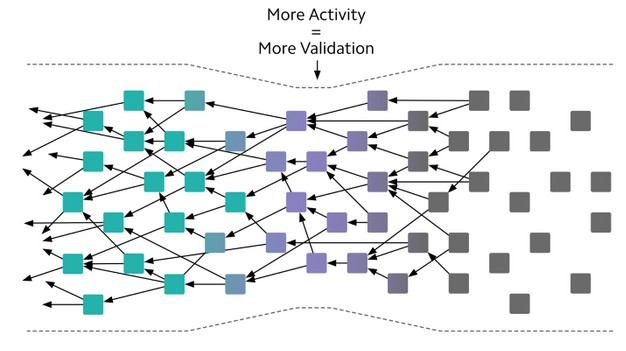
\includegraphics[width=0.8\linewidth]{Figures/Selection_039.jpg}}
\caption{Funcionamiento del Tangle de \cite{tangle_picture}.}
\label{fig:Selection_039}
\end{figure}

\begin{itemize}
\item \textbf{Cuentas} \newline
A diferencia de otras criptomonedas, IOTA no usa un conjunto de clave pública con clave privada para definir una cuenta. Cada usuario posee una semilla, que es un número aleatorio y secreto. Con la semilla se crea una clave pública y una clave privada. La clave pública es usada como destino para fondos. Si el usuario desea gastar los fondos asociados a dicha clave, firma la transferencia con la clave privada correspondiente. Luego, el conjunto de clave pública y privada es descartado y se genera uno nuevo con la semilla secreta. Ese mecanismo se llama esquema de firma única, ya que cada transacción es firmada con una única clave que no se reutiliza.

\item \textbf{Validación} \newline
Para transferir tokens IOTA de una cuenta a otra, hay que seguir los siguientes pasos:
\begin{enumerate}
\item La transacción tiene que ser firmada con claves que todavía no han sido utilizadas.
\item Es necesario elegir y validar dos \textit{tips}: \textit{Tips} son transacciones cuya historia todavía no fue comprobada y se verifica que no existen contradicciones entre ambas transacciones.
\item Se calcula un \textit{Proof of Work} para cada transacción que se publica. De esa forma se evita \textit{spam} en la red.
\end{enumerate}
Luego de completar los pasos descritos, la transacción nueva es publicada como \textit{tip} y otros nodos pueden elegirla para la validación. 

\item \textbf{Costo de transacciones} \newline
Ya que no existen mineros ni forjadores, tampoco existen tarifas de transacciones. El costo de una transacción consiste en el esfuerzo computacional que requiere validar dos \textit{tips} y calcular el \textit{Proof of Work}.
\end{itemize}

IOTA resulta ser una implementación prometedora ya que desafía la arquitectura tradicional del Blockchain e introduce mayores cambios en su funcionamiento. Todavía se encuentra en las etapas tempranas de desarrollo y queda por ver si las mejoras introducidas producen el impacto esperado.


Para la aplicación a implementar, la arquitectura de IOTA presenta los siguientes inconvenientes:

\begin{itemize}
\item El esquema de firma única no permite asignar una identidad única a los participantes de la red.
\item La solución ``Qubic'' para que IOTA soporte \textit{smart contracts} todavía está en desarrollo y no existe una fecha estimativa de lanzamiento. \cite{qubic_roadmap}
\end{itemize}


\section{Lisk}

Lisk es un producto de la Lisk Foundation: CEO Max Kordek y CTO Oliver Beddows quieren implementar un \textit{framework} que ayuda con la creación de Blockchains nuevos - públicos o privados - para una adaptación más simple y rápida de la tecnología.
En mayo del 2016, se lanzó su Blockchain que actualmente permite el intercambio de la criptomoneda LSK y la implementación de aplicaciones descentralizadas, parecido al caso de Ethereum y EOSio. El \textit{framework} que facilita la construcción de un Blockchain propio está en versión alpha y todavía se encuentra en desarrollo.

\subsection{Funcionamiento}

\begin{itemize}

\item \textbf{Cuentas}\newline
Para poder empezar a interactuar con la red de Lisk, es necesario instalar Lisk Hub.
\begin{quote}
Lisk Hub es una solución todo en uno para administrar el ID de Lisk, acceder a los tokens de Lisk, enviarlos así como también para votar a los delegados. Combina la funcionalidad de la antigua billetera y un explorador de Blockchain.\cite{lisk_products}
\end{quote}
A partir de una frase de contraseña secreta se genera un Lisk-Id, un identificador único de la cuenta de usuario. Con dicho Lisk-Id es posible recibir y transferir fondos. Las transacciones tienen que ser firmadas con la frase de contraseña secreta para ser procesadas.

\item \textbf{Validación} \newline
Lisk utiliza \textit{delegated proof of stake} para forjar bloques nuevos.\cite{lisk_consensus} Existen 101 delegados que crean bloques en turno rotatorio y se genera un bloque nuevo cada 10 segundos. Cada bloque incluye 25 transacciones, de modo que Lisk tiene un rendimiento de 2,5 transacciones por segundo. Los delegados cobran un monto de 5 LSK por cada bloque creado y adicionalmente una tarifa por cada transacción incluida en el bloque. Los participantes de la red deben votar a los delegados y pueden recibir un porcentaje de la ganancia del delegado como incentivo de voto.

\item \textbf{Costo de transacciones} \newline
Las transacciones en la red Lisk tienen un costo fijo de 0,1LSK, sin importar el monto que se está transfiriendo.\cite{lisk_transactions} Existe una propuesta para la implementación de tarifas dinámicas pero todavía no se encuentra considerada en el \textit{roadmap} de la implementación. 

\end{itemize}

Para utilizar el \textit{framework}, los futuros implementadores Blockchain pueden descargar las herramientas Lisk Commander, Lisk Core y Lisk Elements, que forma un conjunto de librerías y herramientas que permiten configurar parámetros de un Blockchain propio. El lenguaje principal es Javascript, de esa manera, programadores que provienen de un ambiente de desarrollo web pueden empezar a trabajar con Lisk sin tener que aprender un lenguaje nuevo. Será posible ajustar el mecanismo de consenso, tarifas de transacciones, derechos de accesos, rendimiento como también codificar la aplicación.

Sin embargo, no es la visión de la fundación Lisk que en un futuro haya una multitud de Blockchains aislados entre sí: su objetivo es la interacción entre ``Sidechains''.

 
Sidechains fueron descritos por primera vez en el whitepaper ``Enabling Blockchain Innovations with pegged Sidechains'' donde los autores definen el concepto de la forma siguiente:

\begin{quote}
Proponemos una nueva tecnología, los Sidechains vinculados, que permite transferir Bitcoins y otros activos contables entre múltiples Blockchains.\cite{Back2014EnablingBI}
\end{quote}

Así, un Sidechain es un Blockchain que implementó un mecanismo para poder intercambiar activos con otros Blockchains. Construir aplicaciones en Sidechains tiene varias ventajas:
\begin{enumerate}
\item Es posible definir el mecanismo de consenso y forjado más conveniente para una aplicación.
\item Problemas como errores de código o ataques solamente afectan a un Sidechain.
\item Bienes pueden ser intercambiados entre diferentes Sidechains sin ser convertidos: un Bitcoin en un Sidechain sigue siendo un Bitcoin.
\end{enumerate}

Max Kordek describe su idea para los Sidechains de Lisk de la siguiente manera: 
\begin{quote}
Es posible usar las funcionalidades del Sidechain de otras personas dentro de un Sidechain propio. Por ejemplo, si hay un servicio para enviar mensajes y otro que permite subir imágenes, se pueden aprovechar estas dos aplicaciones para construir una aplicación como una red social, sin volver a implementar la subida de imágenes y el servicio de mensajería. Simplemente se usan otras aplicaciones de Blockchain para eso. Es como un cerebro que evoluciona con cada Sidechain que está conectada al sistema.\cite{youtube_lisk}
\end{quote}

Según el CEO del proyecto, una vez que el \textit{framework} está implementado, será posible implementar un Blockchain privado, adaptar parámetros como costos de transacción y el mecanismo de consenso, e implementar la aplicación que funcione con dicho Blockchain. El \textit{framework} tendría la ventaja para los desarrolladores que mientras ellos se pueden concentrar en escribir la aplicación, Lisk se encargaría de mejorar el funcionamiento de la tecnología Blockchain subyacente. El proyecto tiene aspectos prometedores para el futuro y si su desarrollo estuviese más avanzado, sería considerado como una opción para este proyecto integrador, ya que cumple con los requisitos establecidos.


\section{Hyperledger}

Hyperledger es un proyecto de la Linux Foundation que fue iniciado en diciembre de 2015.
\begin{quote}
El proyecto va a desarrollar un \textit{framework} de código abierto y grado empresarial para \textit{ledgers} distribuidos, con el fin de que desarrolladores se enfoquen en construir aplicaciones robustas y específicas de su industria.\cite{hyperledger_foundation}
\end{quote} 
Los términos \textit{ledger} y Blockchain en este contexto describen el mismo concepto, y más adelante se va a aclarar la diferencia entre ambos.

Una variedad de empresas apoya la iniciativa: en septiembre de 2018 figuran más que 250 miembros en la página web, entre otros Cisco, Hitachi y J.P.Morgan. IBM e Intel aportaron código de trabajos relacionados con Blockchain, lo cual formó la base para los dos proyectos más avanzados: Hyperledger Fabric y Hyperledger Sawtooth.

Desde los inicios de Hyperledger se sumaron una multitud de proyectos. En total hay 5 \textit{frameworks} para diferentes tipos de Blockchains y 5 herramientas que facilitan la interacción y el mantenimiento. En la figura \ref{fig:Selection_051} se ve el enfoque de cada uno.
\begin{figure}[H] % Example image
\center{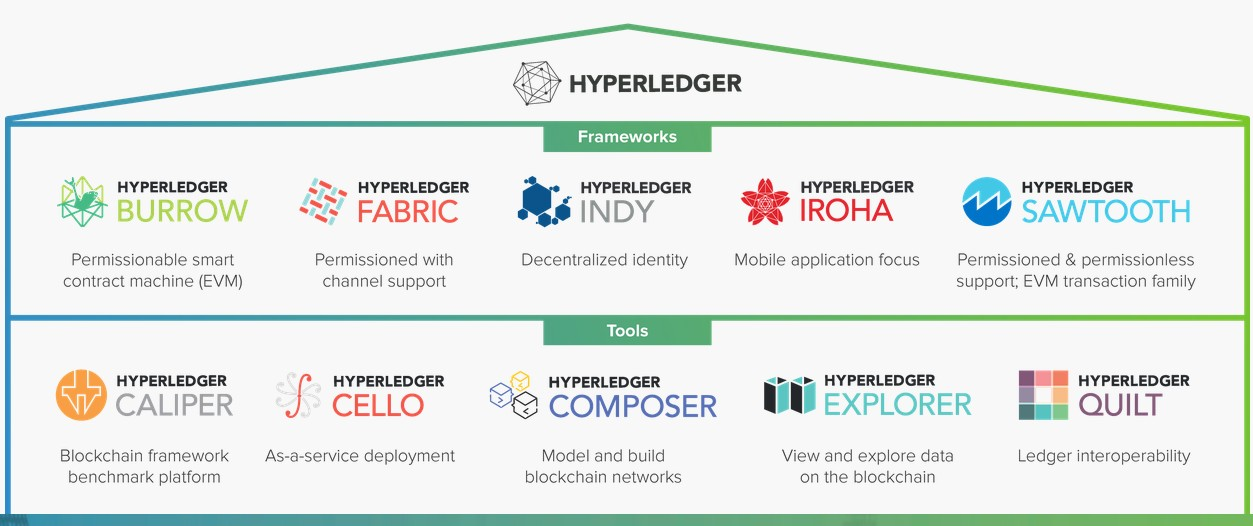
\includegraphics[width=1.0\linewidth]{Figures/Selection_051.jpg}}
\caption{Proyectos en Hyperledger de \cite{hl-projects}.}
\label{fig:Selection_051}
\end{figure}

La mayoría de los proyectos que figuran en \ref{fig:Selection_051} se encuentran en la etapa de incubación, por lo cual su código y su documentación se encuentran incompletos. A continuación se van a describir con mayor detalle los dos proyectos más avanzados, que cuentan con una versión 1.0 y pueden ser usados en producción.

\subsection{Hyperledger Fabric}
Hyperledger Fabric fue el primero de los proyectos Hyperledger y su versión 1.0 se lanzó el 11.7.2017.\cite{hlf_release} Es un \textit{framework} para implementar Blockchains de uso empresarial. Fue diseñado con los siguientes requerimientos:\cite{hlf_whatis}
\begin{itemize}
\item[\textendash] Los participantes tienen que ser identificables.
\item[\textendash] El acceso a la red debe ser autorizado.
\item[\textendash] El sistema necesita alto rendimiento para procesar transacciones.
\item[\textendash] Las transacciones se tienen que confirmar con baja latencia.
\item[\textendash] El sistema debe proveer privacidad y confidencialidad para las transacciones y sus datos relacionados.
\end{itemize}

Los requerimientos especificados se implementaron de la siguiente manera:
\begin{itemize}
\item \textbf{Cuentas} \newline
Organizaciones que participan en el Blockchain hacen uso de una autoridad de certificación - puede ser propia o tercera - para otorgar identidades digitales a sus usuarios. Hyperledger Fabric cuenta con un \textit{Membership Service Provider} y listas de control de acceso: cada identidad digital es verificada con respecto a su validez y sus autorizaciones cuando se conecta a la red.
\item \textbf{Validación} \newline
En Hyperledger Fabric, los nodos que validan transacciones no son los mismos que los nodos que crean bloques nuevos. Así, la carga de procesamiento en la red se distribuye mejor. Además, la división permite la ejecución paralela de transacciones no relacionadas, mejorando así el rendimiento del Blockchain.

\item \textbf{Costo de Transacciones} \newline
Si bien es posible definir una criptomoneda nativa en Hyperledger Fabric, no es necesario y el protocolo de consenso no lo requiere.
\begin{quote}
Fabric puede utilizar protocolos de consenso que no requieren de una criptomoneda nativa para incentivar el minado costoso o para impulsar la ejecución de \textit{smart contracts}.\cite{hlf_whatis}
\end{quote}
 Por ende, las transacciones pueden ser ejecutadas sin pagar una tarifa.
\end{itemize}

\subsection{Hyperledger Sawtooth}
El 30.1.2018, Hyperledger lanzó la versión 1.0 de un segundo proyecto llamado Hyperledger Sawtooth.\cite{hls_release} El código inicial fue aportado por Intel y fue diseñado con los siguientes objetivos:\cite{hls_whatis}
\begin{itemize}
\item[\textendash] Construir una plataforma para \textit{ledgers} distribuidos que sean privados o públicos.
\item[\textendash] Lograr una configuración fina de permisos de accesos y transacciones.
\item[\textendash] Asegurar que \textit{smart contracts} sean seguros.
\item[\textendash] Obtener una separación estricta de la lógica de negocios con la implementación subyacente y facilitar así el desarrollo.
\end{itemize}

El software funciona de la forma siguiente:
\begin{itemize}
\item \textbf{Cuentas}\newline
Con la ayuda de identidades criptográficas se crean roles con determinados permisos. Los clientes interactúan a través de una REST-API con una red de validadores, que verifican los permisos de los clientes y rechazan peticiones si los permisos no son suficientes. Si la petición de una transacción se considera válida, se la envía a un nodo procesador de transacciones para su ejecución. Dichos nodos son los que actualizan el estado del Blockchain.
\item \textbf{Validación} \newline
Como en Hyperledger Fabric, la validación de transacciones y la creación de bloques ocurren en nodos diferentes. Hyperledger Sawtooth ofrece un mecanismo de consenso nuevo llamado \textit{Proof of Elapsed Time}, que aprovecha un ambiente seguro de ejecución en los procesadores Intel. Sin embargo, una característica de Hyperledger Sawtooth es el ``mecanismo de consenso intercambiable'': La forma de llegar al consenso puede ser cambiada por una alternativa proponiendo un cambio a través de una transacción.
\item \textbf{Costo de Transacciones} \newline
Al igual que en Hyperledger Fabric, Hyperledger Sawtooth no  requiere de una criptomoneda para asegurar transacciones y consenso, por lo cual el costo de las transacciones se reduce al costo de procesamiento en la red que requiere cada transacción.
\end{itemize}


Junto con los ya mencionados, Hyperledger Sawtooth provee una cantidad de mecanismos adicionales que distinguen la implementación de Hyperledger Fabric.

Las transacciones se pueden enviar en lotes: se deben ejecutar todas las transacciones de forma exitosa o ninguna. Así se consigue implementar transacciones atómicas como en  bases de datos tradicionales.

Los nodos procesadores de transacciones son capaces de aprovechar paralelismo de transacciones no relacionados, mejorando así el rendimiento del Blockchain.

Hyperledger Sawtooth es compatible con Solidity, es decir \textit{smart contracts} escritos para Ethereum pueden ser ejecutados en Hyperledger Sawtooth con la ayuda de la herramienta Seth. Además, pueden ser testeados en \textit{sandboxes}, ambientes seguros para evitar comportamientos inesperados.

La configuración del Blockchain está guardada en forma de transacciones en el mismo Blockchain, lo cual tiene la ventaja que nodos que son agregados adicionalmente se pueden auto configurar. Además, posibilita modificar el funcionamiento de un Blockchain que ya está en uso: se proponen cambios en forma de transacciones que son aprobados o rechazados en base a un sistema de votos integrado en Hyperledger Sawtooth.


\subsection{Otros proyectos de Hyperledger}

\textbf{Hyperledger Iroha}: Una implementación con un esquema de consenso nuevo que es de alta performance y orientado a dispositivos móviles que se conectan y desconectan con frecuencia de la red. El proyecto todavía está en la versión beta.


\textbf{Hyperledger Burrow}: Es un cliente Blockchain con la máquina virtual de Ethereum integrada. Está diseñado para ejecutar \textit{smart contracts} escritos en Solidity y, para ser usado en un ambiente donde diferentes Blockchains están conectadas entre ellos. Se encuentra en la etapa de incubación. 

\textbf{Hyperledger Indy}: Un \textit{framework} para un Blockchain diseñado para la gestión de identidades digitales. Como Hyperledger Burrow, está en la etapa de incubación.

Otros productos de Hyperledger están pensados para facilitar el desarrollo, como por ejemplo \textbf{Hyperledger Cello}, una herramienta para el despliegue en \textit{clusters} con el fin de ofrecer Blockchain como servicio. \textbf{Hyperledger Caliper} permite realizar \textit{benchmarks} de Blockchains e \textbf{Hyperledger Explorer} posibilita administrar a un Blockchain a través de una interfaz web. Todas las herramientas de Hyperledger se encuentran en etapa de incubación.

Los dos proyectos que se detallaron en esta sección cuentan con las características especificadas para el prototipo. \ref{sec:primeras_especificaciones_prototipo}. Son \textit{frameworks} completamente desarrollados que permiten implementar un Blockchain con las funcionalidades requeridas. De los dos, Hyperledger Fabric se destaca como la opción más conveniente debido a que está específicamente destinado a Blockchains privados y para el prototipo a emplear no se necesita la compatibilidad con Ethereum. Además, emplear \textit{Proof of Elapsed Time} implica una limitación con respecto al \textit{hardware}, ya que el algoritmo solamente funciona en conjunto con arquitectura Intel, por lo cual la mecánica de consenso de Hyperledger Fabric resulta más adecuada.

\section{Conclusiones}
En el mercado existen muchas soluciones para implementar aplicaciones en Blockchain, algunas más desarrolladas que otras. Cada solución tiene su propio enfoque y en el momento de la redacción del informe, la mayoría requieren de un medio de pago en forma criptomonedas. Sin embargo, el código de dichas plataformas suele ser libre y \textit{open source}, por lo cual un equipo de programadores experimentados puede implementar un Blockchain propio haciendo las modificaciones deseadas en un código ya existente.

Para un despliegue de mayor velocidad con un \textit{framework} ya existente, se ofrecen las soluciones de Hyperledger, donde especialmente Hyperledger Fabric e Hyperledger Sawtooth cuentan con un código testeado para ser empleado en ambientes de producción, el soporte de varios lenguajes de programación para aplicaciones y una amplia cantidad de documentación con tutoriales.

Hyperledger Fabric es una solución de código libre que cumple con las siguientes caracterísiticas:

\begin{itemize}
    \item Es una solución pensada para Blockchains privados y Blockchains de Consorcio.
    \item Los permisos de acceso son configurables a través de identidades digitales, que también permiten la implementación de una lista negra para casos de identidades perdidas o robadas. En cada momento, es posible controlar los accesos de lectura y escritura de cualquier entidad.
    \item Si bien el uso de una criptomoneda es posible, el protocolo de consenso no requiere de un incentivo en forma de una criptomoneda.
    \item Los \textit{smart contracts} son fácilmente programables en el lenguaje de programación Golang.
\end{itemize}

Dado que las características mencionadas cumplen con los requerimientos planteados para una solución Blockchain, elaborados en la sección \ref{sec:primeras_especificaciones_prototipo}, se eligió Hyperledger Fabric como \textit{framework} para la implementación del prototipo.

\newpage